\chapter{Urban and Rural Places}

\section{Urbanisation} \label{14/02/2025}
	\subsection{Definition of a Slum}
		\begin{itemize}
			\item Lack of tenure ie. lack of ownership of the land
			\item Sanitation
			\item Durability
		\end{itemize}
	
	\begin{itemize}
		\item Employment
			\begin{itemize}
				\item Governments prefer formal employment because it can be taxed
				\item Informal employment prevents the government from gaining funds to invest in infrastructure and public services
				\item Informal employment lacks safety measures, eg. trash picking job common to developing countries is likely to have poor sanitation, and is not regulated
				\item However, it is more flexible, decreases barriers to employment (paperwork, certification) (also reduces capital and initial investment)
				\item Work outside regulation is not illegal
				\item Can be a source of:
				\begin{itemize}
					\item Child labour
					\item Unsafe working conditions
					\item Environmental concerns
				\end{itemize}
			\end{itemize}

		\item Energy supply
			\begin{itemize}
				\item Power is needed for manufacturing and is necessary to attract foreign investment
				\item People in LICs will buy their own power
				\begin{itemize}
					\item Don't need excessive amounts
					\item Charge a car battery with a solar panel
					\item Known as "leap frogging" technology
				\end{itemize}
			\end{itemize}

		\item Water supply
			\begin{itemize}
				\item Large populations need substantial water supply
				\item Groundwater usage destabilises the soil and causes sinking
				\item Groundwater is also exposed to arsenic and other heavy metals
				\item Water supplies are frequently privatised by city leading to inequality - mismatch of interests from business perspective
			\end{itemize}

		\item Sanitation
			\begin{itemize}
				\item It is hard to use a toilet in a slum
				\item Faecal matter is exposed to the environment
			\end{itemize}
		\item Traffic congestion
			\begin{itemize}
				\item Cycle rickshaws (3 wheeled bike) increase congestion and prevent cars from utilising their speed, causing high inefficiency that also impacts air pollution
			\end{itemize}
	\end{itemize}


	\subsection{Statistics}
		\begin{itemize}
			\item Housing
				\begin{itemize}
					\item Global urban population surpassed rural population in 2007 and is currently at 55\%
					\item 24.2 \% of the urban population lives in slums
					\item By 2030, 1 in 4 people will live in slums, currently, 1 in 7 people live in slums
				\end{itemize}

			\item Pollution
				\begin{itemize}
					\item 99\% of the global population lives in places where air pollution exceeds WHO guidelines
					\item Air pollution is the largest contributor to global disease burden (measured by Disability-Adjusted Life Years (DALYs), where one DALY = one year of good health lost)
					\item 8.1 million premature deaths annually due to air pollution
					\item Traffic congestion costs people in Rio de Janeiro 190 hours per year
				\end{itemize}
			\item Sanitation
				\begin{itemize}
					\item Dharavi has one toilet per 1500 people
				\end{itemize}
			\item Informal economies
				\begin{itemize}
					\item More than 60\% of employed people globally are in informal employment arrangements UNSD-SDG Goals
					\item Up to 92\% of women are in informal employment compared to 87\% for men
				\end{itemize}
		\end{itemize}

		\subsubsection{Case Studies}
			\begin{itemize}
				\item Shanghai
				\begin{itemize}
					\item Increase of over 13 million people from 1987 - 2015
					\item Population density from 1785 - 3809 /km$^2$
				\end{itemize}
			\end{itemize}

\section{Challenges in Rural Places} \label{04/03/2025}

	A clear rural-urban divide exists in most countries

	\begin{enumerate}
		\item Rural areas face challenges in providing adequate and equal healthcare, services, education, and infrastructure
		\item Diminishing economic and social well-being outcomes concentrate poverty and disadvantage in rural places
	\end{enumerate}
	
	Remoteness is measured as a location's proximity to a city.

	Remoteness patterns place Indigenous communities in these areas and further their disadvantage

	\subsection{Provision of Goods and Services}
	
		\begin{itemize}
			\item Rural places often lack a \textbf{population threshold} high enough to provide anything other than low order goods and services (eg. bread, milk)
			\item Larger towns extend their \textbf{sphere of influence} as transport infrastructure and communications technologies improve, as regional centres extend their influence, it makes it harder for smaller towns to support themselves
			\item Automation and economic rationalisation have resulted in job losses in small towns
			\item Population ageing and outward migration exacerbate this decline
				\begin{itemize}
					\item Remote areas have smaller working age populations and more aged people in comparison to major cities
					\item Less people are working, and have smaller taxation revenue
					\item However, old people are hard to keep alive
				\end{itemize}
		\end{itemize}

	\subsection{Provision of Healthcare and Education}
		
		\begin{itemize}
			\item Long distances to hospitals and higher numbers of people per medically trained personnel lead to lower health outcomes
				\begin{itemize}
					\item Regular check-ups are hard to do
					\item People will need to travel long distances to these services
				\end{itemize}
			\item Higher rates of poverty and age result in lower health outcomes
			\item Long distances and isolation result in higher rates of accidents and suicide
				\begin{itemize}
					\item Longer distances to drive increase risks
				\end{itemize}
		\end{itemize}

	\subsection{Provision of Infrastructure}
	
		\begin{itemize}
			\item Lack of communications infrastructure
			\item Fluctuations in economic activity in regional industries make it difficult for infrastructure to efficiently and sustainably underpin long term growth and development (eg. sugarcane is not economically viable in Australia due to overseas competition. Therefore will not be funded by Australian government)
			\item Infrastructure is more expensive per capita in lower density populations
		\end{itemize}

	\subsection{Example Questions}
	
		\begin{enumerate}
			\item \textbf{Describe the reasons for a decline in regional, rural, and remote area populations (approx. 200 words)}

				Variations in population in a particular location occur due to a variety of reasons, predominantly the ability of available services to provide for the population, and the distance of which unprovided resources can be accessed. The accessibility of necessary services such as 


			\item \textbf{Compare and contrast the challenges for regional, rural, and remote area populations in Australia with those globally (approx. 500 words)}
		\end{enumerate}

\section{Mr Ritchie's Lesson} \label{05/03/2025}

	\begin{itemize}
		\item Urban centres serve the population around them
		\item Towns grow to support their populations
		\item Town growth relies on the success on farmers and the townspeople that service these farmers
		\item Farms are now more expensive to run due to technology, ie. less accessible
		\item Horizontal expansion occurs because some farmers cannot compete
		\item Populations to support towns is decreasing
		\item Rural-to-urban migration occurs due to decreasing populations
		\item Christaller's central place theory
		\item Small towns need to support some kind of industry, such as tourism
	\end{itemize}

\section{Understanding Mossman}

	\subsection{Conceptual Map}
	

	\subsection{Timeline}
	
		\begin{itemize}
			\item \textbf{1875} - Dan Hart becomes the first non-indigenous settler in the Mossman district although at that time he did not have tenure
		\end{itemize}


	Mossman Gorge
	Wet tropical area - Luscious green undergrowth
	Buildings with undercover walkways due to rainfall
	Low-rise infrastructure


\section{Nature of Social, Economic, and Environmental Changes in Mossman} \label{18/03/2025}

	\textbf{Social Changes}

		\begin{itemize}
			\item First nation recognition
				\begin{itemize}
					\item Native title established in 2007
					\item Kuku Yalanji bi-lingual signs
					\item Mossman Gorge Cultural Facility
				\end{itemize}
			\item Ageing population
				\begin{itemize}
					\item emigration (18-25)
					\item immigration (55-65)
				\end{itemize}

			\begin{figure}[H]
				\centering
				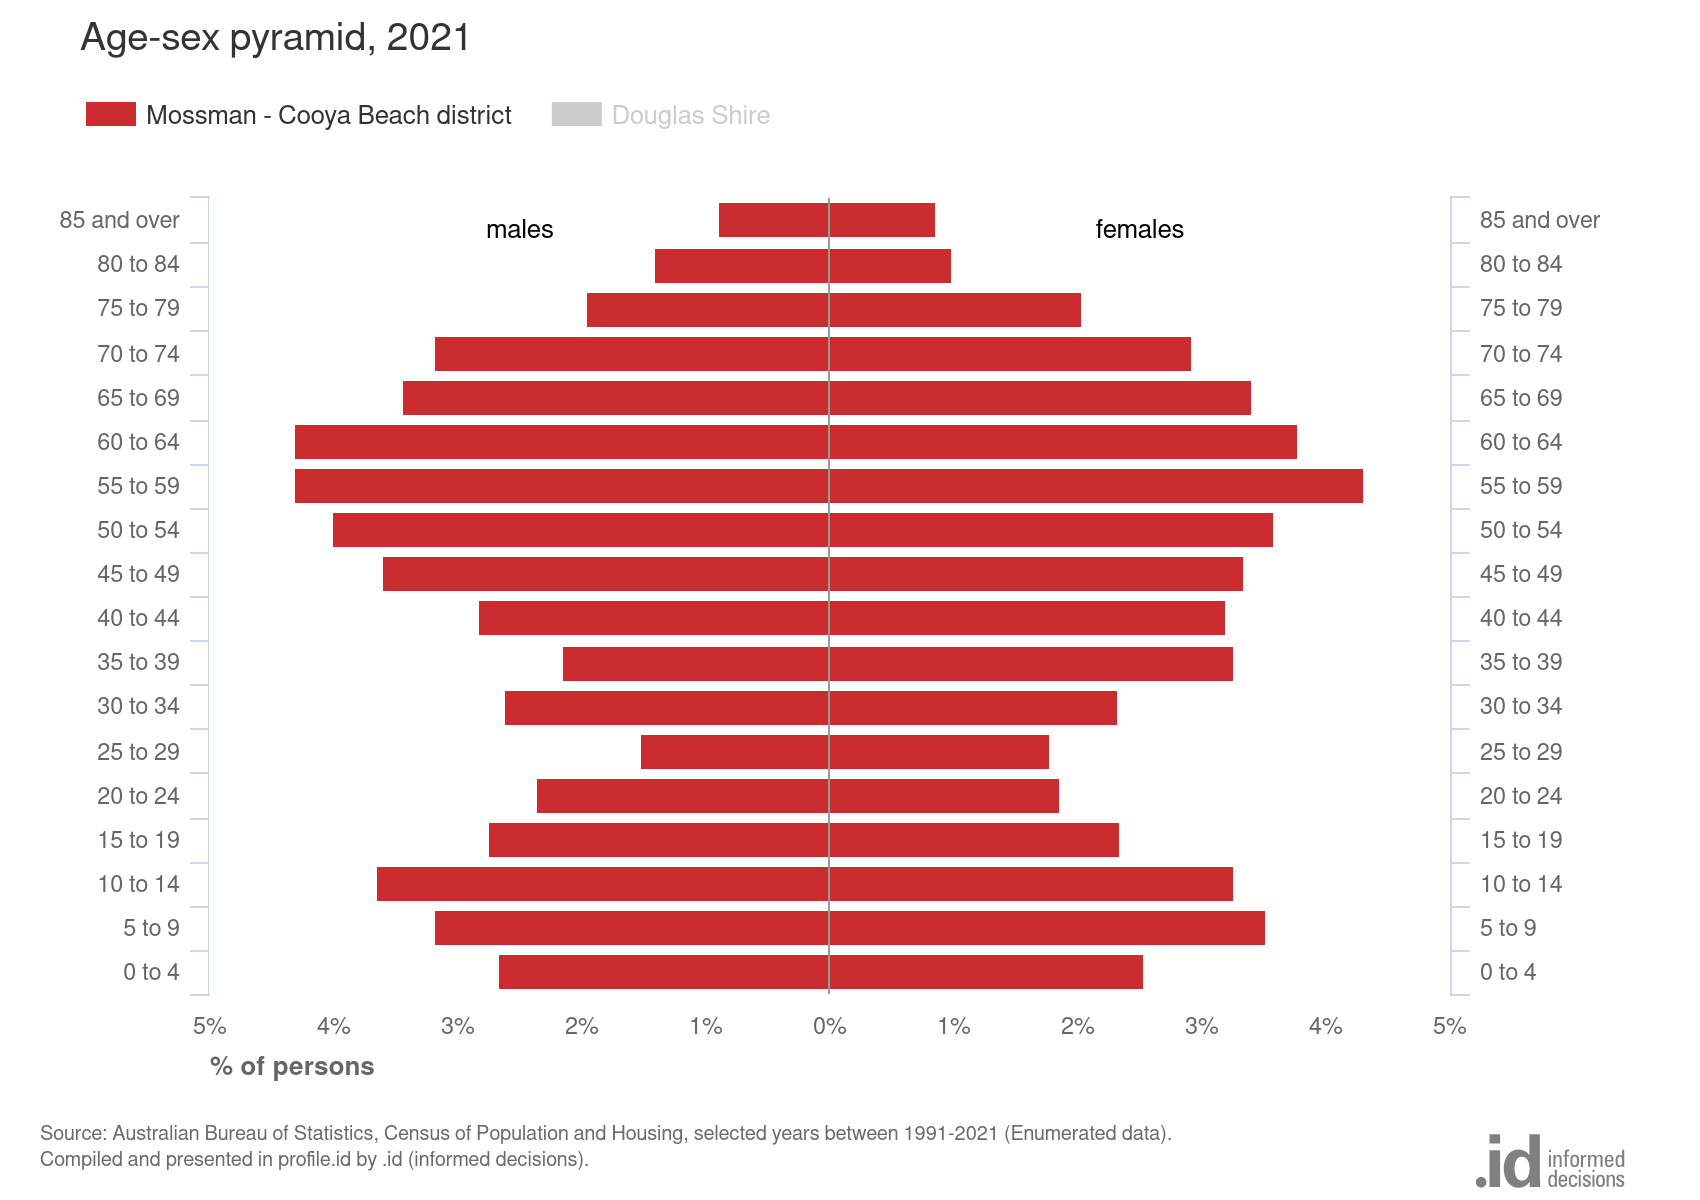
\includegraphics[width=15cm]{mossman_pop_pyramid.png}
			\end{figure}

			\begin{figure}[H]
				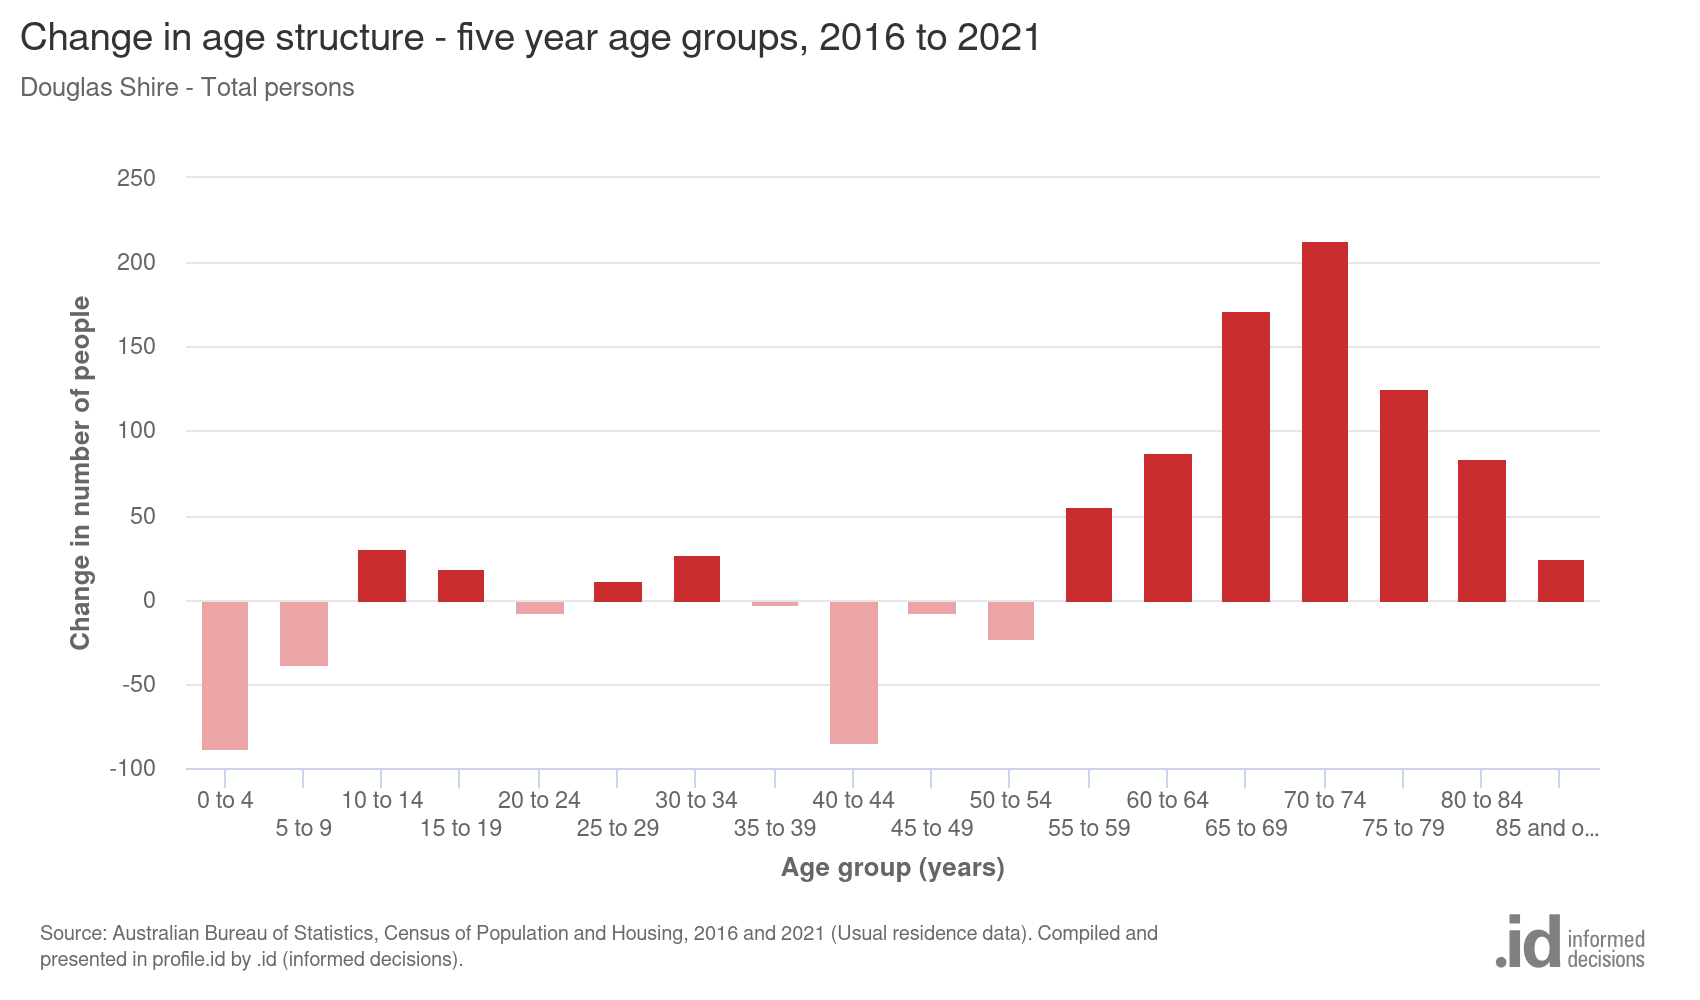
\includegraphics[width=15cm]{5yr_douglasshire_groups.png}
			\end{figure}
		\end{itemize}
	
	\textbf{Economic Changes}
		\begin{itemize}
			\item Sugar industry
				\begin{itemize}
					\item https://www.abc.net.au/news/rural/2024-05-07/mossman-cane-growers-harvest-decision-mill-closure/103806792?utm_campaign=abc_news_web&utm_content=link&utm_medium=content_shared&utm_source=abc_news_web
					\item The Mossman Mill entered voluntary administration in November 2023, and liquidation in February 2024
					\item The closure of the mill is expected to 188 million loss in total economic output and the loss of 575 local jobs
				\end{itemize}
			\item Labour shortage
				\begin{itemize}
					\item Mossman LFPR is at 52.1\%, vs. the national average of 67.3\%
				\end{itemize}
			\item As the sugar industry becomes less sustainable, tourism must grow to compensate
			\item Growth in tourism, tourism development
		\end{itemize}

	\textbf{Environmental Changes}
		\begin{itemize}
			\item Climate change
			\item Prospectus mentions the Daintree Bio Region concept to diversify products and tap into green industry (eg. biofuels), however hasn't been mentioned
		\end{itemize}

	\section{Responses}
		\begin{itemize}
			\item Promotion and diversification of tourism
				\begin{itemize}
					\item Ferry upgrade
					\item Botanic Garden - preservation of local flora
					\item Aquariums can also be used to preserve the reef
					\item Road/cycleway - increase liveability
				\end{itemize}
			\item Promotion and diversification of agriculture
				\begin{itemize}
					\item Diversity in crop
					\item up skilling $\rightarrow$ Daintree Bio Region
				\end{itemize}
			\item Adaptation and mitigation to climate change
				\begin{itemize}
					\item Adaptation
						\begin{itemize}
							\item Microgrids using sugarcane biofuels - this increases the resilience of Mossman
							\item Cooling urban spaces - higher temperatures in a high humidity environment
							\item Biodiversity preservation
						\end{itemize}
					\item Mitigation
						\begin{itemize}
							\item Reef 2050
						\end{itemize}
				\end{itemize}
		\end{itemize}

